\documentclass[preprint,amsmath,amssymb,aps,prd,nofootinbib,floatfix]{revtex4-2}

\usepackage{graphicx}
\usepackage{bm}
\usepackage[nopatch=footnote]{microtype}
\usepackage{mathtools}
\usepackage{amsthm}
\usepackage{url}

\newtheorem{definition}{Definition}
\newtheorem{proposition}{Proposition}
\newtheorem{remark}{Remark}
\newtheorem{assumption}{Assumption}

\DeclareMathOperator{\Law}{Law}
\DeclareMathOperator{\diag}{diag}

\setlength{\emergencystretch}{2em}

\begin{document}

\title{Self-Interacting Dynamics with Exponential Memory:\\
Markovian Embedding, Contractive Memory Fibres, and Metastability Diagnostics}

\author{H. Horn}
\affiliation{Peine Stederdorf, Germany}

\date{26 July 2026}

\begin{abstract}
This technical note specifies the mathematical structure used by a companion
numerical study of self-interacting stochastic dynamics with exponential
forgetting.
A visible state $x_n$ is coupled to a deposited memory field $\rho_n$.
The visible trajectory is generally non-Markovian, while
$z_n=(x_n,\rho_n)$ is a time-homogeneous Markov process.
We derive the exact exponential-memory expansion, prove contraction of the
affine memory fibre along a common visible path, distinguish one-step
invertibility from loss of the ordered history, and state a formal continuum
scaling.
We also formulate control-aware metastability diagnostics without asserting
that the current scalar model has isolated a nonlinear metastable state.
The note is intended as a technical appendix or companion reference, not as a
standalone novelty claim or numerical phase study.
\end{abstract}

\maketitle

\section{Introduction}

Self-interacting stochastic processes couple a trajectory back to a summary of
its past.
Classical examples include reinforced processes, Brownian polymers, true
self-avoiding or self-repelling motion, and self-interacting diffusions
\cite{Pemantle2007,DurrettRogers1992,AmitParisiPeliti1983,
TothWerner1998,PelitiPietronero1987}.
Bena\"im, Ledoux, and Raimond use a normalized cumulative occupation measure;
for symmetric interactions, Bena\"im and Raimond prove convergence toward the
critical set of a nonlinear free-energy functional
\cite{BenAImRaimond2002,BenaimRaimond2005}.
Herrmann and Roynette study an unnormalized interaction with the full past and
establish convergence or boundedness in particular one-dimensional
self-attracting cases \cite{HerrmannRoynette2003}.

Those results do not directly transfer to the model below because its history
is exponentially discounted and represented by a deposited spatial field.
The closest current comparison is the aging-kernel model of Mili\v{s}i\'c,
Meunier, and Roux, which treats weighted linear interactions with past
positions and includes an explicitly solvable exponential-memory case
\cite{MilisicMeunierRoux2026}.
Generalized Langevin and Mori--Zwanzig constructions provide the broader
principle that memory equations can become local after the state is augmented
\cite{Mori1965,Zwanzig2001,JaganathanValani2025}.

The claims of this note are consequently structural and modest.
The specific object is a discrete point process coupled to a nonlinear
potential generated by a deposited memory field.
For this object we make the normalized and finite-measure conventions
explicit, prove the direct Markov and contraction statements, and specify what
would count as metastability beyond a linear relaxation cloud.
We do not prove ergodicity, a spectral gap, a nonlinear bifurcation, or the
existence of a separate knot phase.
\section{Discrete Model}

Let $\Omega\subseteq\mathbb{R}^d$ be an effective state space with reference
measure $dx$. The Euclidean structure is used only to write kernels,
gradients, and diagnostics; it is not identified with physical space. Let
$G_\sigma$ be a smooth normalized deposition kernel of width $\sigma$, and
let $K$ be an interaction kernel for which the convolution
\[
(K*\rho)(x)=\int_\Omega K(x,y)\rho(y)\,dy
\]
is differentiable in the regimes considered below.

\begin{assumption}[Baseline regularity]
Let $\Omega\subseteq\mathbb{R}^d$ be Borel and equip it with a boundary or
extension convention that keeps $x_{n+1}$ in $\Omega$.
Assume $G_\sigma\in L^1(\Omega)$, $G_\sigma\geq0$, and
$m_G=\int_\Omega G_\sigma<\infty$.
The noise law is a Borel probability measure with finite second moment.
For every finite memory measure reached by the recursion,
$K(x,y)$ is measurable in $(x,y)$, continuously differentiable in $x$, and
$\nabla_xK(x,\cdot)$ is integrable against that measure; the resulting drift
is Borel measurable.
For the formal continuum and Hessian approximations we additionally require
local Lipschitz and growth bounds on the drift and the corresponding second
$x$-derivatives of $K$ near the linearization region.
\end{assumption}

The discrete process is
\begin{align}
x_{n+1}
&=x_n+\varepsilon\xi_n-\eta\nabla\Phi_n(x_n),
\label{eq:xupdate}\\
\rho_{n+1}(x)
&=(1-\lambda_{\mathrm m})\rho_n(x)
+\beta G_\sigma(x-x_{n+1}),
\label{eq:rhoupdate}\\
\Phi_n(x)&=(K*\rho_n)(x),
\label{eq:potential}
\end{align}
where $0<\lambda_{\mathrm m}<1$, $\beta\geq0$, $\varepsilon\geq0$,
$\eta\geq0$, and $\xi_n$ are independent centered noise variables, typically
taken isotropic with unit covariance. The parameter $\lambda_{\mathrm m}$ is
the forgetting rate, while $\beta$ is the deposited memory strength. The
previously used normalized convention is the special case
$\lambda_{\mathrm m}=\beta=\alpha$.

Let $m_G=\int_\Omega G_\sigma(x)\,dx$ and $M_n=\int_\Omega\rho_n(x)\,dx$.
Then
\begin{equation}
M_{n+1}=(1-\lambda_{\mathrm m})M_n+\beta m_G.
\label{eq:massrecursion}
\end{equation}
Thus the stationary total retained memory mass, when the scalar recursion is
stable, is $M_*=\beta m_G/\lambda_{\mathrm m}$. Unit mass is preserved only in
the normalized case $m_G=1$, $M_0=1$, and $\beta=\lambda_{\mathrm m}$. If
$\rho_0$, $G_\sigma$, and $\beta$ are nonnegative, every $\rho_n$ is
nonnegative. The choice $\beta=\lambda_{\mathrm m}$ is therefore a useful
density normalization, not a structural requirement; an overall memory scale
can often be absorbed into $K$ or $\eta$.

The project term ``knot'' is reserved for a nonlinear metastable regime that
survives comparison with the linear center-relative mode and matched controls.
Compact motion around a moving memory center alone is called a localized
memory cloud and does not meet that criterion.

\section{Exponential Memory and Contractive Fibres}
\label{sec:memory}

The memory equation can be unrolled exactly.

\begin{proposition}[Exponential memory representation]
For $n\geq1$,
\begin{equation}
\rho_n
=(1-\lambda_{\mathrm m})^n\rho_0
+\beta\sum_{j=0}^{n-1}(1-\lambda_{\mathrm m})^j
G_\sigma(\,\cdot-x_{n-j}).
\label{eq:memoryexpansion}
\end{equation}
\end{proposition}

\begin{proof}
The claim follows by induction. For $n=1$ it is exactly
Eq.~\eqref{eq:rhoupdate}. If it holds at $n$, then
\[
\begin{aligned}
\rho_{n+1}
&=(1-\lambda_{\mathrm m})^{n+1}\rho_0\\
&\quad+\beta\sum_{j=1}^{n}(1-\lambda_{\mathrm m})^j
G_\sigma(\cdot-x_{n+1-j})\\
&\quad+\beta G_\sigma(\cdot-x_{n+1}),
\end{aligned}
\]
which is Eq.~\eqref{eq:memoryexpansion} with $n+1$.
\end{proof}

The deposited weights are
\begin{equation}
w_j=\beta(1-\lambda_{\mathrm m})^j.
\end{equation}
Their relative tail is controlled by $\lambda_{\mathrm m}$, independently of
the deposition scale $\beta$. For a rest-weight threshold $\delta$, the
effective memory depth satisfies
\begin{equation}
j_\delta=\frac{\log\delta}{\log(1-\lambda_{\mathrm m})}
\sim\frac{|\log\delta|}{\lambda_{\mathrm m}}
\quad(\lambda_{\mathrm m}\ll1).
\label{eq:memorydepth}
\end{equation}
Thus $\lambda_{\mathrm m}^{-1}$ is the natural update-count scale for memory
persistence. Figure \ref{fig:memoryweights} shows the normalized convention
$\beta=\lambda_{\mathrm m}=\alpha$ for representative values of $\alpha$.

\begin{figure}[tbp]
\centering
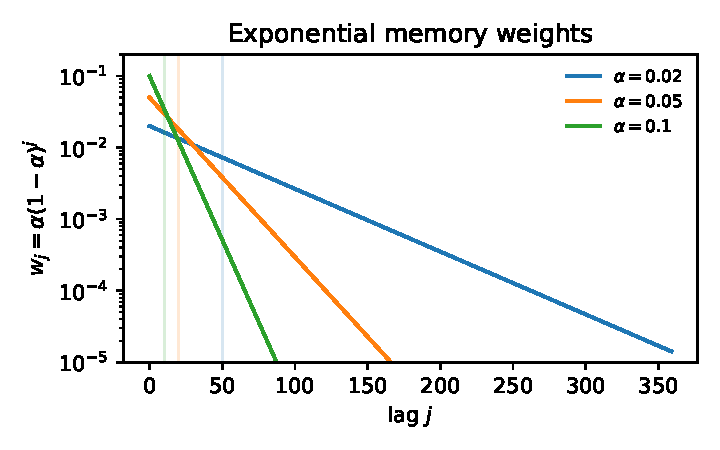
\includegraphics[width=0.7\linewidth]{fig_memory_weights.pdf}
\caption{Normalized exponential memory weights $w_j=\alpha(1-\alpha)^j$, corresponding to $\beta=\lambda_{\mathrm m}=\alpha$. Vertical guide
lines mark $j=\lambda_{\mathrm m}^{-1}=\alpha^{-1}$ for each curve.}
\label{fig:memoryweights}
\end{figure}

\begin{proposition}[Pathwise memory-fibre contraction]
Fix a common visible trajectory $x_1,\ldots,x_n$. Let $\rho_k$ and
$\tilde\rho_k$ solve Eq.~\eqref{eq:rhoupdate} with the same deposited kernels
but different initial memory fields. Then
\begin{equation}
\rho_n-\tilde\rho_n=(1-\lambda_{\mathrm m})^n(\rho_0-\tilde\rho_0).
\label{eq:fibrecontraction}
\end{equation}
Consequently, for any homogeneous norm on the memory space,
\begin{equation}
\|\rho_n-\tilde\rho_n\|=(1-\lambda_{\mathrm m})^n\|\rho_0-\tilde\rho_0\|.
\end{equation}
\end{proposition}

\begin{proof}
Subtract the two memory recursions. The deposited kernels cancel because the
visible trajectory is common:
\[
\rho_{k+1}-\tilde\rho_{k+1}
=(1-\lambda_{\mathrm m})(\rho_k-\tilde\rho_k).
\]
Iterating gives Eq.~\eqref{eq:fibrecontraction}.
\end{proof}

This contraction is a statement about the memory fibre under a fixed visible
path. It is not yet a global contraction theorem for the full feedback system,
because different memory fields can alter future positions through
Eq.~\eqref{eq:xupdate}. A full contraction analysis must control the coupled
pair $(x_n,\rho_n)$.

\section{Markovian Embedding}
\label{sec:markov}

Define the augmented state
\begin{equation}
z_n=(x_n,\rho_n)\in\Sigma.
\end{equation}
Given $z_n$ and a fresh noise draw $\xi_n$, Eqs.~\eqref{eq:xupdate} and
\eqref{eq:rhoupdate} determine $z_{n+1}$. Thus the augmented dynamics is a
time-homogeneous Markov process.

\begin{definition}[Transition kernel]
For measurable $A\subseteq\Sigma$ define
\begin{equation}
P(z,A)=\mathbb{P}\{z_{n+1}\in A\mid z_n=z\}.
\end{equation}
The observable Markov operator is
\begin{equation}
(Uf)(z)=\int_\Sigma f(z')P(z,dz')
=\mathbb{E}[f(z_{n+1})\mid z_n=z].
\label{eq:operator}
\end{equation}
\end{definition}

The operator $U$ is linear, positive, and unital: $U1=1$. Its iterates satisfy
$U^{m+n}=U^mU^n$. In the stochastic case it is generally not multiplicative:
$U(fg)$ need not equal $(Uf)(Ug)$. The correct algebraic object is therefore
a positive unital Markov operator on observables, with a dual action on
probability measures, rather than a deterministic algebra automorphism.

\begin{proposition}[Visible non-Markovian projection]
The projected process $x_n$ is generally not Markov.
\end{proposition}

\begin{proof}
Take the same visible position $x$ with two memory fields $\rho$ and
$\tilde\rho$ such that
\[
\nabla(K*\rho)(x)\neq\nabla(K*\tilde\rho)(x).
\]
Then the conditional next-step laws of $x_{n+1}$ differ because their drift
terms in Eq.~\eqref{eq:xupdate} differ. Hence conditioning on $x_n=x$ alone
does not determine the next-step law.
\end{proof}

The memory update should not be described as algebraically noninvertible in
isolation. If $x_{n+1}$ and $\rho_{n+1}$ are known and $\lambda_{\mathrm m}\neq1$, then
\[
\rho_n=\frac{\rho_{n+1}-\beta G_\sigma(\cdot-x_{n+1})}{1-\lambda_{\mathrm m}}
\]
is a formal rearrangement. The precise irreversibility statement is different:
the present augmented state does not generally encode the full ordered
history, and the stochastic dynamics defines a forward Markov semigroup rather
than a reversible group action.

% Skew-product terminology is omitted because no result below uses it.
\section{Formal Continuum Approximation}

Let $t=\lambda_{\mathrm m} n$ and consider a joint scaling
\[
\begin{gathered}
\lambda_{\mathrm m}\to0,\qquad \varepsilon\to0,\qquad
\frac{\varepsilon^2}{2\lambda_{\mathrm m}}\to D,\\
\frac{\eta}{\lambda_{\mathrm m}}\to\gamma,
\qquad \frac{\beta}{\lambda_{\mathrm m}}\to\kappa.
\end{gathered}
\]
The final scaling assumption keeps the memory source finite; the normalized
case has $\kappa=1$. Formally, the visible coordinate approaches
\begin{equation}
dX_t=-\gamma\nabla(K*\rho_t)(X_t)\,dt+\sqrt{2D}\,dW_t,
\label{eq:sde}
\end{equation}
while the memory field satisfies
\begin{equation}
\partial_t\rho_t=\kappa G_\sigma(\cdot-X_t)-\rho_t.
\label{eq:memoryode}
\end{equation}
More generally one may introduce a memory time $\tau$ and write
\[
\partial_t\rho_t=\tau^{-1}\left(\kappa G_\sigma(\cdot-X_t)-\rho_t\right),
\]
equivalently
\[
\rho_t=\kappa\tau^{-1}\int_{-\infty}^{t}e^{-(t-s)/\tau}
G_\sigma(\cdot-X_s)\,ds
\]
after transients. The extended process $(X_t,\rho_t)$ is local in the scaled
time variable and Markovian; the visible process $X_t$ alone retains memory.

Equations \eqref{eq:sde}--\eqref{eq:memoryode} are a formal effective
description, not a convergence theorem in this paper. A rigorous limit would
require specifying topology, tightness estimates, regularity of $K$, boundary
conditions, and the scaling of $\Omega$ if the domain changes with $\lambda_{\mathrm m}$.

\section{Metastability and Knot Diagnostics}

A candidate knot is a long-lived localized feedback regime in the augmented
dynamics. Operationally, for a region $\mathcal{K}\subseteq\Omega$ one can
track retained memory mass
\begin{equation}
M_n(\mathcal{K})=\int_{\mathcal{K}}\rho_n(x)\,dx.
\end{equation}
Persistence over many memory times,
\[
\Delta n\gg\lambda_{\mathrm m}^{-1},
\]
is a minimal diagnostic for metastability, not a proof of a new particle-like
object.

Several diagnostics are useful and mutually constraining:
\begin{itemize}
\item residence-time statistics of $x_n$ in candidate regions;
\item retained memory weight $M_n(\mathcal{K})$;
\item autocorrelation functions of positions and reduced memory features;
\item local linearization near a metastable center $x_*$;
\item slow modes of a transfer-operator estimate on augmented features.
\end{itemize}

For local linearization, suppose a metastable regime has slowly varying memory
$\rho$ and a center $x_*$ with $\nabla(K*\rho)(x_*)=0$. With
\[
H=\nabla\nabla(K*\rho)(x_*)
\]
the continuum approximation becomes locally
\begin{equation}
dX_t=-\gamma H(X_t-x_*)\,dt+\sqrt{2D}\,dW_t.
\end{equation}
Positive eigenvalues of $\gamma H$ give local relaxation rates in stable
directions. A relaxation-based stability scale can be written as
\[
\Gamma_{\rm rel}=\tau_{\rm rel}^{-1},\qquad
\widehat\Gamma=\frac{\sigma^2}{D}\Gamma_{\rm rel}.
\]
This is a mass-like or stability proxy only. It is not a calibrated physical
mass and should not be identified with $mc^2$.

\subsection{Transfer-Operator View}

Let $\psi(z_n)$ be a reduced feature vector for the augmented state, for
example position, memory centroid, current offset from the memory centroid,
memory spread, retained memory mass, or learned/PCA/Fourier features of
$\rho_n$. A finite-rank Ulam or Markov-state approximation estimates a
transition matrix at sample lag $\ell$ from pairs
\[
(\psi(z_n),\psi(z_{n+\ell})).
\]
Let $\tau_\ell$ denote the update-time or scaled-time lag represented by those
pairs. For finite trajectories, states that are observed only as terminal
lagged targets have no empirical outgoing row. The reference implementation
reports how many such rows are handled and, by default, treats them as
absorbing in the finite matrix. Eigenvalues with modulus numerically equal to
one are still reported in the spectrum but are not converted into relaxation
rates. Production analyses should check the terminal-row count, vary the lag
and discretization, and compare against independent residence diagnostics.
Slow non-unit eigenvalues $\lambda_i(\tau_\ell)$ then give implied rates
\begin{equation}
\Gamma_i(\tau_\ell)=-\frac{1}{\tau_\ell}\log|\lambda_i(\tau_\ell)|.
\label{eq:impliedrates}
\end{equation}
Almost-invariant sets and coherent sets are then candidate metastable knots
\cite{FroylandLloydSantitissadeekorn2010}. Related variational and Koopman
approaches are standard in molecular kinetics and operator-theoretic model
reduction \cite{NoeNuske2013,NoeWuPrinzPlattner2013,WilliamsKevrekidisRowley2015,KlusEtAl2018}.

Figure \ref{fig:transferspectrum} shows one small reproducible transfer
spectrum from the companion pipeline. It is an illustration of the diagnostic
workflow, not evidence for a universal phase diagram.

\begin{figure}[tbp]
\centering
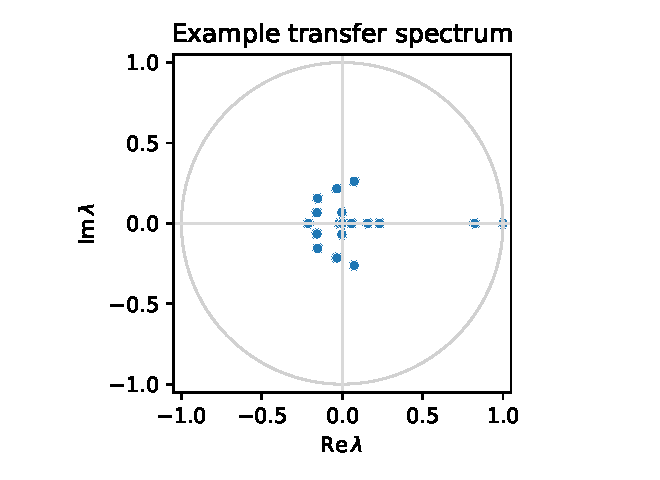
\includegraphics[width=0.58\linewidth]{fig_transfer_spectrum.pdf}
\caption{Example eigenvalues of a finite-state transfer estimate from reduced
augmented features. Non-unit modes close to the unit circle are candidates for
metastable structure, subject to lag-time choice, discretization, finite-sample row
handling, and sampling checks.}
\label{fig:transferspectrum}
\end{figure}

% Numerical implementation details are maintained with the companion study.
\section{Relation to Existing Literature}

The normalized occupation measure of Bena\"im, Ledoux, and Raimond weights the
past cumulatively as $t^{-1}\int_0^t\delta_{X_s}\,ds$.
Their convergence and free-energy results, including the symmetric-interaction
theory of Bena\"im and Raimond, therefore concern a different time dependence
from Eq.~\eqref{eq:rhoupdate}
\cite{BenAImRaimond2002,BenaimRaimond2005}.
Herrmann and Roynette use the unnormalized full-history drift
$\int_0^t\Phi(X_t-X_s)\,ds$ and prove strong localization statements for
specific one-dimensional interactions \cite{HerrmannRoynette2003}.
This is an important nearby localization result, but it is not an
exponential-memory model.

Mili\v{s}i\'c, Meunier, and Roux introduce an aging kernel for linear
self-interaction and analyze general convolution weights as well as a
particular exponential case \cite{MilisicMeunierRoux2026}.
This is the closest temporal-memory comparison found in the present review.
The model here differs by using a deposited spatial density and allowing a
nonlinear kernel-induced force, but the general ideas of aging and exponential
state closure are shared.
Accordingly, novelty cannot rest on exponential forgetting or Markov
augmentation alone.

Mori--Zwanzig and generalized Langevin methods provide the broader embedding
principle \cite{Mori1965,Zwanzig2001,JaganathanValani2025}.
Transfer operators and Markov-state models provide standard diagnostics for
slow processes and almost-invariant sets
\cite{NoeNuske2013,NoeWuPrinzPlattner2013,
WilliamsKevrekidisRowley2015,KlusEtAl2018}.
The value of the present note is the explicit specification and separation of
these ingredients for the companion scalar model, not a new general embedding
theorem.
\section{Open Mathematical Problems}

The structural results above do not settle the main hard questions. The
following are open tasks:
\begin{itemize}
\item well-posedness of the continuum approximation under explicit kernel and
state-space assumptions;
\item Feller properties and invariant measures for the augmented Markov
process;
\item Lyapunov/Harris drift conditions of the form
$PV\leq\lambda V+b$ outside compact sets \cite{MeynTweedie2009};
\item conditions for uniqueness, geometric ergodicity, and spectral gaps;
\item coupled contraction estimates for $(x_n,\rho_n)$, not only the memory
fibre under a fixed path;
\item bifurcation and metastability regimes for attractive, repulsive, and
two-scale attractive-repulsive kernels;
\item convergence and bias analysis for transfer-operator estimates on
reduced memory features.
\end{itemize}

\section{Boundaries}

The structural results do not imply a nonlinear knot phase, dimension
selection, a hard finite signal speed, Lorentz invariance, quantum dynamics,
particle structure, or calibrated masses.
A finite propagation bound would additionally require local transfer and the
absence of direct long-range response.
Dimension-selection claims require ambient-dimension controls and a diagnostic
that does not simply reproduce isotropic covariance rank.
Relaxation rates remain model diagnostics unless an independent physical
calibration is supplied.
\section{Conclusion}

The model defines a self-interacting stochastic process with exponential
forgetting and a field-mediated self-potential. The visible trajectory is
generally non-Markovian, but the explicit memory field yields a Markovian
augmented dynamics. The memory fibre is affine and pathwise contractive for a
common visible trajectory. These structural facts make localization and
metastability testable, but they do not prove a nonlinear metastable regime.
The note supplies the mathematical reference needed to formulate and falsify
such a claim in the companion numerical study.

\bibliographystyle{apsrev4-2}
\bibliography{references}

\end{document}
